\documentclass[10pt,a4paper]{article}
\usepackage[utf8]{inputenc}
\usepackage[english]{babel}
\usepackage[square, numbers, sort&compress]{natbib}
\usepackage[pdftex]{graphicx}   %para eps
\usepackage{epstopdf}          %para eps
\usepackage{float}
\usepackage{amsmath}
\usepackage{verbatim}
\usepackage{amsfonts}
\usepackage{amssymb}
\usepackage{lscape}
\usepackage{longtable}
\usepackage{booktabs}
\usepackage{eurosym}
\usepackage{pdfpages}
%\usepackage{graphicx}
\usepackage{subfig}
%\usepackage{media9}
\usepackage{color}
\usepackage{fancyhdr}
\usepackage{lastpage}	
\usepackage{parskip}
\usepackage[scaled]{helvet}
\usepackage{blindtext}
\usepackage{sectsty}
\usepackage{multicol}
\usepackage{enumitem}
\usepackage{multirow}   %tabla
\usepackage{colortbl} %colores tabla
%\usepackage[table]{xcolor} %colores tabla
\usepackage{rotating}  %rotating
\usepackage{scrextend} %footnote
\usepackage{natbib}
\usepackage{arabtex}
\usepackage{utf8}
\usepackage{array}
\usepackage{xr}
\externaldocument{path/to/external-file1}
\externaldocument{path/to/external-file2}
%\usepackage[svgnames]{xcolor}
\usepackage[labelfont={color=LibrelloColor,bf}, labelsep=period]{caption}
\renewcommand*{\familydefault}{\sfdefault}
\usepackage[left=1.75cm,right=1.75cm,top=1.75cm,bottom=3.75cm]{geometry}
\usepackage{titlesec}
\usepackage{svg}
\usepackage{flushend}
\PassOptionsToPackage{normalem}{ulem}
\usepackage{ulem}
	\providecolor{added}{rgb}{0,0,1}
	\providecolor{deleted}{rgb}{1,0,0}
	%% Change tracking with ulem
	\newcommand{\added}[1]{{\color{added}{}#1}}
	\newcommand{\deleted}[1]{{\color{deleted}\sout{#1}}}
\usepackage{setspace}
\usepackage[hyphens]{url}
\usepackage{siunitx}
\usepackage[T1]{fontenc}

% Green - CiS, OF
%\definecolor{LibrelloColor}{RGB}{0,85,0}
% Red - JoHS
\definecolor{LibrelloColor}{RGB}{128,0,0}


\usepackage[hidelinks, urlcolor=LibrelloColor]{hyperref}
\urlstyle{same}
\raggedcolumns
\flushcolumns
\usepackage{etoolbox}
\usepackage{caption}
%\usepackage{subcaption}
\usepackage{supertabular}
\usepackage{booktabs}
\usepackage{microtype}
\usepackage{threeparttable}
\usepackage{doi}
\usepackage{balance}
\usepackage{enumitem}
\usepackage{eurosym}

\usepackage[color=yellow,icon=Comment,hoffset=-10mm, author=Librello Editorial's Office]{pdfcomment}

\titleformat{\section}
{\color{LibrelloColor}\normalfont\bfseries\filright}
{\color{LibrelloColor}\thesection.}{0.5em}{}

\titleformat{\subsection}
{\color{LibrelloColor}\normalfont\itshape\filright}
{\color{LibrelloColor}\thesubsection.}{0.5em}{}

\titleformat{\subsubsection}
{\color{LibrelloColor}\normalfont\itshape\filright}
{\color{LibrelloColor}\thesubsubsection.}{0.5em}{}

\usepackage{array} %criando coluna de largura fixa alinhada a esquerda
\newcolumntype{L}[1]{>{\raggedright\let\newline\\\arraybackslash\hspace{0pt}}p{#1}}
%criando coluna de largura fixa alinhada a direita
\newcolumntype{R}[1]{>{\raggedleft\let\newline\\\arraybackslash\hspace{0pt}}p{#1}}
\renewcommand{\arraystretch}{1.3}
\titlespacing\section{0pt}{12pt}{12pt}
\titlespacing\subsection{0pt}{12pt}{12pt}
\titlespacing\subsection{0pt}{12pt}{12pt}	
\renewcommand*{\refname}{References and Notes}

\fancypagestyle{document}{
	\renewcommand{\footrulewidth}{0pt}
	\renewcommand{\headrulewidth}{0pt}
	\renewcommand{\footrulewidth}{0pt}
	\renewcommand{\headrulewidth}{0pt}
	\renewcommand{\footskip}{40pt}
	\cfoot{\normalfont\thepage}
	\rhead{}\lhead{}
}

\fancypagestyle{firstpage}{
	\renewcommand{\footrulewidth}{0pt}
	\renewcommand{\headrulewidth}{0pt}
	\renewcommand{\footrulewidth}{0pt}
	\renewcommand{\headrulewidth}{0pt}
	\renewcommand{\footskip}{70pt}
	%CiS
%\lhead{Challenges in Sustainability $\mid$ 2016 $\mid$ Volume 4 $\mid$ Issue 1 $\mid$ Pages \thepage--\pageref{LastPage} \\DOI: 10.12924/cis2016.040100XX\\
%	ISSN: 2297--6477}
%	\rhead{\includegraphics[height=0.59in]{CiS.eps}}
	%JoHS
	\lhead{Journal of Human Security $\mid$ 2021 $\mid$ Volume 17 $\mid$ Issue 1 $\mid$ Pages \thepage--\pageref{LastPage} 
	\\DOI: 10.12924/johs2021.17010091\\
	ISSN: 1835--3800}
	\rhead{\includegraphics[height=0.59in]{JoHS.eps}}
	%OF
	%\lhead{Organic Farming $\mid$ 2018 $\mid$ Volume 3 $\mid$ Issue 1 $\mid$ Pages \thepage--\pageref{LastPage} \\DOI: 10.12924/of2018.030100XX\\
	%ISSN: 2297--6485}
	%\rhead{\includegraphics[height=0.59in]{OF.eps}}	

	\lfoot{\footnotesize © 2021 by the authors; licensee Librello, Switzerland. This open access article was published\\ under a Creative Commons Attribution License (\url{http://creativecommons.org/licenses/by/4.0/}).}
	\cfoot{}
	\rfoot{\vspace*{-24pt}\includegraphics[height=0.49in]{librello.eps}}
}

\newcommand{\beginsupplement}{%
        \setcounter{table}{0}
        \renewcommand{\thetable}{A\arabic{table}}%
        \setcounter{figure}{0}
        \renewcommand{\thefigure}{A\arabic{figure}}%
     }

\makeatletter
\def\NAT@def@citea{\def\@citea{\NAT@separator}}
\makeatother


\begin{document}


\flushcolumns
\raggedcolumns



\pagestyle{document}
\thispagestyle{firstpage}


\vspace*{70pt}

\setlength{\parindent}{0cm}
%\textit{Research Article}
\textit{Review}
\vspace*{-12pt}

\begin{center}
\line(1,0){500}
\end{center}

\vspace*{12pt}
\begin{flushleft}
\begin{LARGE}
\textbf{{\color{LibrelloColor} A Systematic Literature Review of Gendered Human Security Approaches}} 
\end{LARGE}

\vspace*{12pt}

Theresa A. Ammann$^{1,}$* and Tamara A. Kool$^{2,3}$

\vspace*{6pt}

$^1$ Department of Anthropology, Aarhus University, H{\o}jbjerg, Denmark \\
$^2$ Maastricht Graduate School of Governance, Maastricht University, Maastricht, The Netherlands \\
$^3$ Maastricht Economic and Social Research Institute on Innovation and Technology, United Nations University, Maastricht, The Netherlands

\vspace*{6pt}

* Corresponding author: tamara.kool@maastrichtuniversity.nl; Tel: +31 6 15285810

\vspace*{6pt}

Submitted: 13 October 2020 $\mid$ In revised form: 13 September 2021 $\mid$ Accepted: 14 September 2021 $\mid$ \\
Published: 23 December 2021
\end{flushleft}
\setcounter{page}{91}


\vspace*{-18pt}
\begin{center}
\line(1,0){500}
\end{center}

\vspace*{12pt}
%\vspace{\baselineskip}

\begingroup\leftskip= 1cm\rightskip 1cm

%\vspace*{10pt} %
%\vspace*{8pt}
\textbf{{\color{LibrelloColor}Abstract:}} \textls[-20]{While many have argued for Human Security to integrate a gendered perspective, there is a lack of a consistent approach which hampers the transformative potential that otherwise could be achieved.  To better understand how gender has been incorporated in relation to gender, we therefore conducted a systematic review of the literature that combined feminist approaches and Human Security from 1994 (Human Security's inception) to June 2018. In exploring this literature, the following questions were addressed: (a) How is criticism and support of Human Security framed in feminist research? (b) How are gender and feminist research (values) defined in relation to Human Security? (c) Which feminist approaches to Human Security are taken? (d) How do these feminist approaches dismiss or support Human Security and which trends emerge? We found that most studies solely focus on integrating women in the Human Security debate, while men, masculinities, and/or causes of structural inequalities and insecurities remain unaddressed. Studies that address structural inequalities and discuss both men and women come from critical feminist and intersectional backgrounds. We conclude that most gendered approaches to Human Security still need to fully incorporate feminist approaches to be able to truly challenge global gendered inequalities and insecurities.}

\textbf{{\color{LibrelloColor}Keywords:}} feminist studies; gender; human security; security studies; systematic review

\par\endgroup

\setlength{\parindent}{0.5cm}
\setlength{\parskip}{0cm}
\setlength{\bibsep}{0cm}

\vspace*{10mm}
%\clearpage
\begin{multicols}{2}

\section{Introduction}

\noindent In a widely cited special issue on Human Security in 2004, the editors argued that Human Security (HS) \citep{R1} had come to a halt before it had even realized its potential \citep{R2}. Challenging this debate, Hoogensen and Stuv{\o{}}j \citep{R3} argued that taking a gendered perspective would allow HS to realize its potential. Both seek to challenge the notions of power and identity. By recognizing gender dynamics, the ``relational and power positions of various identities'' (\cite{R3}, p.~225) can be unfolded by bringing in a critical bottom-up perspective. By including a gendered perspective, context, relationality and intersubjectivity which affect insecurities can be further explored  \citep{R3,R4}. In turn, this would allow for a move to an equitable and inclusive society where all are included. Nonetheless, literature continues to take diverging perspective towards its understanding gender and its integration into human security. Inspired by Hoogensen and Stuv{\o}j's argument \citep{R3}, this article therefore sets out to examine how gender has been used in conjunction to HS. To this end, we reviewed the literature on gender and HS since HS' emergence in 1994 until June 2018 with the following two research questions in mind: Which feminist approaches to Human Security are taken? And to what extent has the literature developed a (uniform) gendered HS approach? By understanding how the debate on gender and human security has developed over time, we aim to contribute to a more nuanced discussion that allows human security to be truly inclusive of the different experience of the individuals.

To answer these research questions, we employed a systematic literature review to assess and synthesize the existing literature on HS and gender in a consistent and as objective possible manner. Through the review we address the following sub-questions: \\
\noindent a) How is Human Security framed in feminist research? \\
b) How are gender and feminist research (values) defined in relation to Human Security? \\
c) Which feminist approaches to Human Security are taken? \\
d) How do these feminist approaches dismiss or support Human Security and which trends emerge? \\
\textls[-15]{By asking these questions we seek to establish to what extent scholars have formulated a uniform gendered HS approach and if any trends can be discerned. We conclude by outlining possible implications of our findings for a gendered HS approach. Before setting out the analysis, we set out an overview of the methodological approach taken as well as a brief summary on the studies that comprised our dataset.}

\section{Methodology}

\noindent \textls[-20]{To assess how scholars have combined Human Security and gender (research), we adopted a systematic literature review approach, which is a qualitative approach that allows us to analyze a large amount of studies and map them alongside various categories. It adopts a systematic approach to addressing the literature that seeks to limit the bias on the side of the author that otherwise may influence reviews \citep{R5}. In our study, we seek to understand firstly, which approaches to human security have been taken, and secondly, how gender has been conceptualized in the studies, and lastly, how the gendered HS approach is informed by the feminist approaches and approaches towards HS \citep{R6}. To date, we have not come across a similar systematic literature review on this topic. This section first sets out the protocol for the systematic literature review based on the guidelines outlined by Petticrew and Roberts \citep{R5}  (see \textbf{Appendix A} \ref{Appendix A} for a flow diagram). Next, it discusses the methodological approach taken before briefly describing the sample of studies.}

\subsection{A Step-Wise Approach to the Systematic Literature Review} 

\noindent \textls[-30]{Since we sought to identify the general feminist/gendered approach to HS, we firstly determined search strings to find the literature in various repositories. We searched for studies that featured a combination of ``human security'' and a gender-related idiom in their title, which included any of the following terms: gender, gendering, engendering, gendered, women, woman, men, man, feminism, feminist, femininity, masculinity.  The underlying assumption is that a study that features these keywords in the title is more likely to focus on these topics in detail and seek to contribute to the specific discussion. We would like to recognize that this may result in a potential bias as the author may perceive human security as a relevant topic for study and thus may not necessarily take a critical approach towards human security. Further,we realize that this search query may have excluded studies that actually address HS and gender but do not indicate this in their title. Nonetheless, we posit that the search criteria are warranted as we  focus on studies that dealt with these topics explicitly rather than merely peripherally.}

Secondly, only studies written in English, categorized as grey and peer-reviewed literature (e.g., articles, books, edited volumes, chapters from editorial books), and published between 1994 and 2018 were included. This cut-off point was chosen as UNDP first introduced Human Security in their 1994 \textit{Human Development Report} \citep{R7}.

With these inclusion criteria in mind, we searched the following databases: Google Scholar, Google Books, Web of Science, Scopus and JStore. As each database is constructed differently, we need to recognize that the compiled literature is by no means exhaustive, and studies may have been left out. Also, by using multiple search strings and various databases, sources may come up several times. These searches were conducted at two moments in time: first, between October 7 and November 4, 2016, and the second search was conducted on July 5, 2018 \citep{R8}. In total, 429 entries were identified.

\textls[-20]{Following this search, we checked the results \textit{within} each database and identified double entry sources. This were subsequently removed. Consequently, 108 studies were excluded during this step. We then inspected the studies more closely and removed studies that did not feature our inclusion keywords in the title (N = 14) or were written in a foreign language although their title and abstract were written in English (N = 9). Furthermore, we only included peer-reviewed articles, books, chapters, working papers and PhD theses that were available in print or online. Accordingly, we removed book reviews, I/NGO reports, flyers, conference papers, op-eds and unavailable studies (N = 110). Lastly, eight edited volumes and single chapters came up in the search engine. To avoid double counting, we included the individual chapters and excluded the edited volume. Consequently, we were left with a total of 180 studies.}

Following the first stage exclusion, we compiled the remaining studies and again removed double-entries (N = 52). This left us with a total of 128 studies that remained subject to the inclusion/exclusion criteria as part of the second stage exclusion. 

\textls[-20]{The inclusion and exclusion criteria part of the second stage were defined according to the theoretical considerations underpinning the research design set out above, as well as quality assurance. In terms of quality assurance, this led to the exclusion of three articles due to their poor English academic standard. As for the theoretical considerations, we are interested in he usage of Human Security as a paradigm and approach that was conceived by the UN in 1994, rather than a general description of the security of humans that is not linked to the HS paradigm as outlined by the UN in 1994.Therefore, we distinguished between \textit{Human Security} the paradigm (we referred to this as \textit{``HS''}) and human security as denoting the security of humans (we referred to this as \textit{``hs''}). This resulted in the exclusion of twenty-three sources. Further, if the article only includes HS or gender as a byline and do not discuss these in further detail, the study was also excluded (N = 10).  In total, thirty-six studies were excluded during this phase.}

As we came across three chapters in the previously identified edited volumes which fulfilled our selection criteria that had not been identified during the initial searches, we decided to included them as well. This left us with a total of ninety-five articles to be reviewed for a complete reference list of the sample.

\subsection{Methodological Approach}

\noindent \textls[-20]{This study employs a narrative analysis \citep{R5} to determine to what extent heterogeneity is present within the literature when it comes to gender and HS. Each study was analyzed according to the following categories: definitions of gender; understanding of gender/feminist research; definitions of HS; stance on HS; and gendered HS approach taken.---\textbf{Appendix B} \ref{Appendix B} illustrates a sample analysis for three articles.}

\textls[-27]{Next, we further analyzed the classifications to be able to answer the identified sub-questions. This phase consists of three stages. Firstly, each category was coded according to its definitions. These codes were next grouped together to identify emerging patters. Secondly, ``gender'' and ``gender or feminist research'' were compared as this additional layer of clustering allowed for an in-depth understanding of emerging trends. Lastly, the category identified as ``Approach to Human Security and gender'' assessed how studies' definitions of gender and gender research overlapped with their understanding of HS.}

\textls[-20]{Through the analysis, similarities and differences in the literature became apparent. The systematic literature review firstly, allows for a closer examination on how HS has been envisioned by various authors. Secondly, it sets out the approaches taken towards gender and how this reflects different strands of feminist approaches. Lastly, it allows us to relate the conceptualization of gendered HS or lack thereof, back to the underlying theoretical foundations.}

\subsection{Describing the Sample}

\noindent \textls[-20]{Our sample comprised a diverse dataset, although some characteristics were more prevalent than others (see \textbf{Appendix B} \ref{Appendix B} for an overview of all sample characteristics). The majority of studies were chapters and articles that based their research on theoretical data sources, and secondary and primary qualitative data, in the form of informants. If based on qualitative data, the sample size was often not mentioned. As most studies applied a universal level of analysis, it is not surprising that most studies did not specify their geographical focus. Those with a more specific geographical focus tended to focus on Sub-Saharan Africa and Southeast Asia by either taking a regional or national level of analysis. Our dataset therefore largely originates from academic circles, is largely theoretical and qualitative, and takes a more universal perspective.}

\textls[-20]{In terms of distribution over time, most studies were published between 2004 and 2014 (see Figure \ref{Fig1}). Due to the limited sample size and the general academic publication climate (e.g., slow publication processes, academic pressures), it is difficult to hypothesize what caused this peak and what led to its decline. Nonetheless, the United Nations Security Council Resolution 1325, passed in 2000, resulted in an increased attention to women-peace-and-security-related issues in academic and policy circles, which may explain part of the increase in publications.}

\end{multicols}

\noindent \begin{minipage}{\columnwidth}
\centering
\resizebox{0.85\columnwidth}{!}
%\resizebox{\columnwidth}{!}
{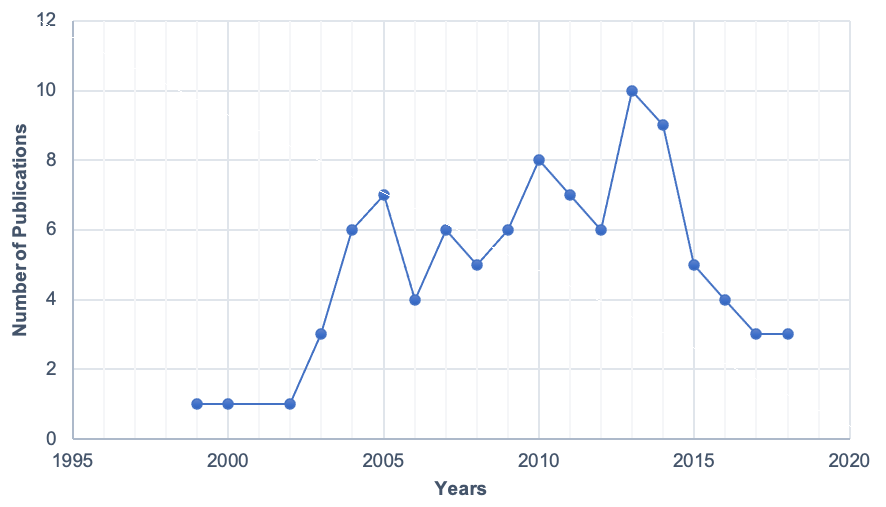
\includegraphics[width=1\textwidth]{Fig1.png}}
\captionof{figure}{Publications over the years.} 
\label{Fig1}
\end{minipage}
\vspace{\baselineskip}

\begin{multicols}{2}

\section{Approaches to HS 1994 to 2018}

\subsection{Identified HS Definitions}

\noindent \textls[-5]{In line with Alkire \citep{R9}, we found no prevalent definition of HS, instead multiple definitions of HS prevailed. So while we were able to identify numerous overarching characteristics, we found it impossible to pinpoint one definition that could be representative of HS within the academic debate. Generally, HS is used to refer to a variety of components that are generally linked to political, economic, and social structures that consequently ensure the achievement of human security with some arguing the need to go beyond these securities and include all threats to human security (see \citep{R10}). Without understanding the complexity and the various facets that are referred to when conceptualizing HS, it is difficult to contextualize the term. To do so, two elements are worthwhile to discuss in more detail, namely the role of the state and the transnational nature of human security.}

Firstly, the role of the state in bringing about human security should be considered. While a holistic definition of HS recognizes a bottom-up approach alongside the state's responsibility to ensure human security, only a small number of articles explicitly address this. While HS may be seen as an alternative, addition or impediment to national security, the state has the main responsibility to bring about human security. Again, this aspect may relate back to the human rights angle as well as the security discourse in general. Thus, by never fully embracing the bottom-up perspective and the inclusion of civil society, it seemingly fails to disentangle itself from a more narrow approach to HS. 

This brings to the foreground a more general challenge, namely the underlying transnational character of human security. While HS concerns the security of the individual and its community, many issues that affect the human go beyond borders, e.g., pandemics, environmental disasters, conflicts. To address these issues, one often looks towards the international community and state actors. Subsequently, the importance of considering power dynamics and holding patriarchal institution accountable should be underlined if one wants to achieve human security \citep{R11,R12}. This in turn links back to the local-global dynamics and interconnected dynamics, all of which makes feminist approaches more valuable as they address the underlying (unequal) structures of human security. 

To analyze the identified HS definitions more systematically, each study was assigned an overarching HS-definition category. In this, we followed Tadjbakhsh and Chenoy (\cite{R13}, p.~121) who argue that HS definitions fall on a scale that increasingly becomes more holistic. That is, definitions can be placed on a scale that becomes increasingly more holistic as the definitions move---from left to right---from solely advancing the (a) freedom from critical fear to include (b) freedom of \textit{critical want} to include (c) freedom to \textit{enlarged want} to finally include (d) the freedom to live life in dignity, which is the most \textit{holistic} definition of HS. HS definitions that focus on \textit{critical fear} are therefore most closely related to more narrow traditional national security definitions that place more emphasis on the role of the state; e.g. Canada's HS understanding or studies that focus on the Responsibility to Protect. HS definitions that focus on critical want and enlarged want straddle the center of the scale and are increasingly broader, more holistic, and human rights focused  (\cite{R13}, p.~47).\textit{Critical want} seeks to ensure people's basic needs, while \textit{enlarged want} takes this one step further by ensuring access to choices and therefore enables one's capabilities. The broadest HS definitions are most \textit{holistic}  and as such do not only advance all freedoms of want and fear but call for the freedom to achieve these in dignity; e.g., the \textit{HS Now} report and the 1994 UNDP report promote HS as a people-centered approach that ensures human development and promotes human rights and a life in dignity.

Accordingly, we found that the studies' HS definitions were distributed along this scale as follows: 3 studies called for \textit{Critical fear} HS definitions, 8 for \textit{Critical want}, 34 for \textit{Enlarged want}, and 50 called for \textit{Holistic} definitions. When examining the distribution over the years (see Figure \ref{Fig2}), we found that \textit{Critical fear} and \textit{Critical want} definitions had marginally decreased, \textit{Enlarged want} definitions had significantly decreased, and \textit{Holistic} definitions had significantly increased. Thus, it emerges that there is a general trend towards a more holistic understandings of HS in the literature.

\end{multicols}

\noindent \begin{minipage}{\columnwidth}
\centering
\resizebox{1\columnwidth}{!}
%\resizebox{\columnwidth}{!}
{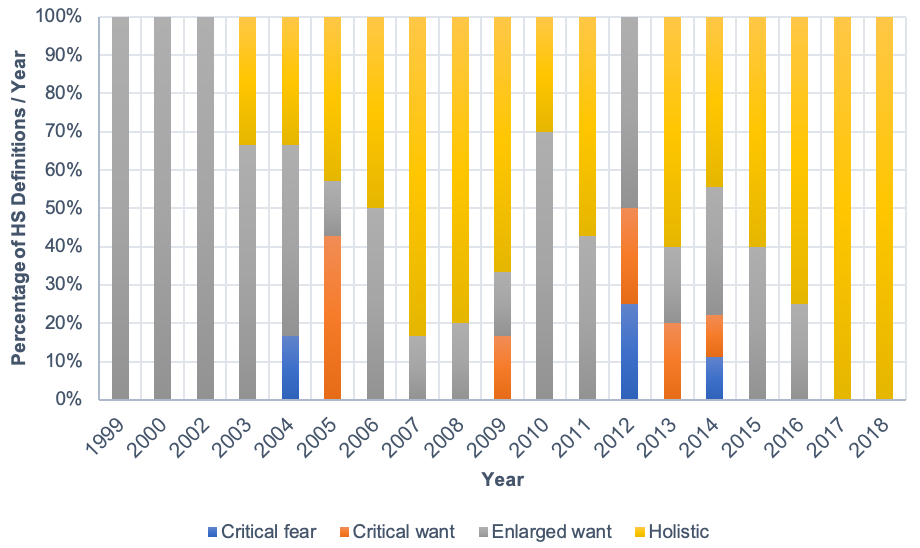
\includegraphics[width=1\textwidth]{Fig2.png}}
\captionof{figure}{Distribution of overarching HS definitions over the years.} 
\label{Fig2}
\end{minipage}
\vspace{\baselineskip}

\begin{multicols}{2}

\subsection{Nuancing Human Security}

\noindent \textls[-20]{Human Security has the potential to account for a ``cosmopolitan formulation of security and as theoretical and practical tool for peace'' (\cite{R14}, p.~87). It has the potential to bridge different strands of security scholars (such as feminists security studies, critical theory and the Copenhagen School) in ``new and potentially transformative ways'' due to their common normative assumptions (\cite{R15}, p.~37). Though this is not necessarily agreed upon by all as another argued that HS was no novel contribution to security studies (see \citep{R16}) and may even perpetuate a neoliberal perspective (see \citep{R17}).}

\textls[-20]{In their discussion on Human Security the majority of authors place critical notes alongside HS. These notes pertain to primarily to the inclusion of a gendered or feminist perspective (N = 41) (e.g. \citep{R3,R18,R19,R20,R21}) and to a lesser extent recognition of ethics of care \citep{R22},  and power and empowerment (see \citep{R23,R24}). Additionally, some call for HS studies to be grounded in ethnography that clarified the position of the researcher to avoid overlooking research subjectivities \citep{R10,R25,R26}.}

\textls[-20]{Importantly, three articles that criticize the conceptualization of Human Security argue that women's security is not equal to people's security, a discussion that can be linked back to early feminist debates on ``who counts as human.'' They question whose perspective is included and who is excluded \citep{R4,R27,R28}. This feminist discussion of who is included in discussions relating to human security is taken up in several studies. As Marhia \citep{R4} states, ``human'' implies a referent object of security, provided subjectivity, exclusion and social status are sufficiently considered. Ellen Lammers \citep{R10} draws out another often excluded security perspective, namely the security of refugees. Unlike national security, HS has the possible ability to advance gendered security dimensions and make audible the voices of those marginalized or most vulnerable, as well non-citizens. Only one article specifically refers to the human security of citizens \citep{R14}, whereas several others refer to those affected by conflict and displacement \citep{R10,R11,R29}.}

\textls[0]{HS furthermore needs to be cognizant on the role of the state. Some even indicate that if HS is co-opted by the state, this may result in further polarization of civil society which would in turn prevent the attainment of a gender equal society \citep{R11,R30,R31}.}

\textls[-20]{The above analysis showcases that most studies call for a more detailed discussion of themes such as power, empowerment, women, gender dimensions, the role of the state and a more detailed account of researcher's positionality. Their definitions of HS, however, are not uniform within the reviewed literature. Since certain components of power, gendered structures, patriarchy and neoliberal perspectives can perpetuate human \textit{insecurity}, it is essential to explore HS in relation to gender to establish the various gendered HS approaches that studies have taken over the years. Therefore, we next set out to examine the respective feminist studies approaches taken and the conceptualization of gender, and how these relate to each other.}

\section{Gendered Approaches from 1994 to 2018}

\subsection{Identified Feminist Studies Subcategories}

\noindent In this section, we identified the studies' feminist subcategories either based on their explicit self-identified subcategory (N = 40) or by assigning them a subcategory that they drew upon most in their study, if the authors did not explicitly self-identify themselves. The more critically and directly the studies were engaged with feminist literature, the more likely they were to self-identify with a feminist subcategory. For example, the most critically and radically engaged form of feminism, Postmodern Feminism, was self-identified (N = 5), whereas for the least critical form of feminist research, Mainstream Feminism, only 1 author self-identified. 

Before we provide a more detailed account of the distribution of these feminist subcategories, a clearer explanation of our understanding of these subcategories is warranted. In total, we identified eight such subcategories: \textit{Mainstream Feminism, Mainstream Feminism drawing on Feminist Security Studies (FSS), Critical Feminism, Postcolonial Feminism, Third World Feminism, Poststructural Feminism, Postmodern Feminism, and Ecofeminism.}

The least critical approach of them is \textit{Mainstream Feminism}, which seeks the equality of men and women by focusing on the plight of women, e.g., Gender-Based Violence (GBV). Mainstream Feminism does not integrate established, critical feminist approaches and scholars, and does not integrate social categories such as race and class \citep{R32}. \textit{Mainstream Feminism---FSS} is similar to Mainstream Feminism's focus but differs in that it has its analytical base in Feminist Security Studies. \textit{Mainstream Feminism}---FSS does not engage with feminist research and often only focuses on the UNSCR 1325, which addresses the need to protect women and seeks to integrate women in peacebuilding processes based on their assumed inherent mothering peacefulness. The focus on the dichotomy between men and women is precisely where Mainstream Feminist approaches (i.e., both \textit{Mainstream Feminism} and \textit{Mainstream Feminism---FSS}) differ from more critical feminist approaches that places a larger importance on the differences \textit{within} male and female groups. Therefore, many Mainstream Feminists draw on gender stereotypes that in turn are rejected by critical approaches. 

\textit{Critical Feminism}, on the other hand, draws on intersectionality and thereby addresses inequalities that are results of power-imbalances along the lines of identities, such as gender, ethnicity, race, religion, sexuality, etc. As such, Critical Feminist approaches often align with the understandings and approaches of \textit{Postmodern} and/or \textit{Poststructural Feminism}. It regards feminism as an issue of not only gender but other identities of oppression. \textit{Postcolonial Feminism} is similar to Critical Feminism's approach (i.e., intersectionality) but it focuses on the needs of indigenous people (often women) who have been marginalized. It is therefore heavily engaged with issues of racism and colonialism. \textit{Third World Feminism} is similar to Postcolonial Feminism's focus but differs in that it insists on indigenously defined understandings of feminism. \textit{Poststructural Feminism} is heavily inspired by Judith Butler's work and regards gender as a social construct of an interplay of language, sociology, subjectivity and power-relations. Poststructural Feminism often engages in literary analyses as it tends to focus on discourses. \textit{Postmodern Feminism's} understanding of gender is the same as Poststructural Feminism's although Postmodern Feminism is more radical in its approach and goals. It seeks to undo society's patriarchal norms by rejecting all gender essentialism, falsifying gendered dichotomies, and promoting subjectivities to highlight diversity and difference within groups of men and within groups of women, rather than solely looking at differences between these groups.

Finally, \textit{Ecofeminism} sees the historic abuse and domination of women and the environment as comparable as both have been exploited and regarded as helpless. As such, ecofeminists argue that true equality cannot be achieved for as long as someone/something is treated as subordinate, including the environment. This category can be seen as separate from critical and mainstream approaches.

Interestingly, the studies are evenly split into two overarching feminist camps: critical and mainstream feminist approaches (both comprise 46 studies). Only 3 studies were classified as \textit{Ecofeminism}. When examining the classifications in more depth, we conclude that most studies draw on an intersectional approach in their analysis (\textit{Critical Feminism}, N = 27) or take a more mainstream feminist approach that is rooted in FSS (N = 26), with the remaining twenty drawing on \textit{Mainstream Feminism}. On the other hand, we find that more critical approaches are taken more rarely: \textit{Postcolonial Feminism} (N = 8), \textit{Postmodern Feminism} (N = 5), \textit{Poststructural Feminism} (N = 3), and \textit{Third World Feminism} (N = 3).

Over time, studies drawing on \textit{Critical Feminism} and \textit{Mainstream Feminism drawing on FSS} have steadily increased, whereas studies from Mainstream Feminist backgrounds have slightly decreased. Finally, studies from all other branches have remained static and minimal over the years. This indicates an increased interest in drawing on established critical feminist approaches and/or mainstream feminist security studies.

\subsection{Identified Understandings of Gender}

\noindent When analyzing the author's understanding of gender, we applied the same principles as we did for analyzing the studies' subcategory of feminist studies. In about half of the studies, the authors' understanding of gender was explicitly defined. For the other half, we assigned understandings of gender based on their application of the word gender. When looking at all studies, we found that the majority of studies used gender to refer to and focus solely on women; thirty-four studies used gender to refer to both women and men, and only two studies focus on men. Both studies that focus on men and masculinity either do so in the context of displacement in Tanzania \citep{R29} or in Iraqi conflict \citep{R17} and its effect on perceived masculinity.

When we examined the how the understanding and focus of ``gender'' developed over time, we observed that in general the focus on women increased over the years, whereas a focus on both men and women decreased slightly. This increase in the focus on women is likely related to the fact that Mainstream Feminism drawing on FSS (which largely uses ``gender'' to focus on women) has continued to increase over the years.

\subsection{How Feminist Studies Subcategories Understand Gender}

\noindent The more a study engages with critical feminist approaches, the more its usage of gender moves from ``women'' to ``both genders.'' Similarly, the majority of critical feminist studies reflects on the gender stereotypes and roles of both women and men; with the exception of studies drawing on Postcolonial and Third World Feminisms where the majority focuses on women (see \citep{R33}). We assume that a study's focus on women when referring to gender can largely be attributed to that study's respective wider field continuing to struggle to include women. For example, \textit{Mainstream FSS} focuses on women because the wider security studies field continues to neglect women in its analyses; for example, Chenoy \citep{R34} argues that national security (studies) is a patriarchal construct that needs to be challenged by focusing on the security of women. Critical feminist approaches (i.e., \textit{Critical Feminism, Poststructural Feminism}, and \textit{Postmodern Feminism}) on the other hand, have gone beyond the inclusion of women and instead focus on both genders to investigate how gender is enacted. For example, Natalie Hudson \citep{R21} categorically challenges and rejects the widespread misuse of ``gender'' as ``women'' and Heidi Hudson \citep{R22} shows that this misuse blurs out not only the importance of masculinities but also the vast varieties of in-group differences amongst women and men. Accordingly, studies drawing on the most critical approach, \textit{Postmodern Feminism}, exclusively focus on both genders. Lastly, \textit{Critical Feminism} is the only approach that includes studies focusing solely on men. This can be seen as a counterbalance to the persistence of less critical feminist approaches that focus on women alone. The next section seeks to understand how the feminist studies subcategories relate back to the different gendered HS approaches taken in the literature.

\section{Gendered HS Approaches from 1994 to 2018}

\subsection{Overview of Approaches}

\noindent Having examined all studies, we identified six overarching gendered HS approaches which the studies had taken: thirty-seven studies called for a gendering of the HS paradigm by providing a \textit{Gender Approach to HS}, twenty called for a \textit{Gender as an Add-on} to HS analyses, sixteen percent were interested in the \textit{HS of Women}, thirteen regarded \textit{Gender as inherent to HS}, eight provided a \textit{Feminist Critique of HS}, and only one article believed \textit{HS was a tool to advance feminist agendas}. 

In general, we found that the identified gendered HS approaches fell into two overarching categories: (a) approaches that were more gender-aware (i.e., \textit{Gender Approach to HS, Gender as an Add-on}, and \textit{Feminist Critique of HS}), and (b) approaches that were less gender-aware (i.e., \textit{HS as a tool to advance feminist agendas, HS of Women, and Gender as inherent to HS}). More gender-aware approaches drew on feminist themes, issues, principles, guidelines and/or theories; while their less gender-aware counterparts tended to focus on women's issues alone without drawing on feminist theories to make their argument. 

Studies that advocate for a \textit{Gender Approach to HS} do so in numerous ways: a gendering of HS to avoid a perpetuation of existing gendered structures (see \citep{R28}), an inclusion of intersectional theories in HS analyses (see \citep{R35}), a feminist perspective that investigates ``who'' is included when politicians and scholars speak of ``humans'' (see \citep{R20}), a revival of HS from a postmodern feminist perspective (see \citep{R36}), and the inclusion of discussions about masculinities as well as femininities to account for victimized men and agentic women \citep{R17}. Although these studies call on different means or particular aspects of feminist research, all of them do so to bring about a more specific and systematic \textit{Gender Approach to HS}. To exemplify, the analysis on homeworkers in Thailand by Sasaki et al. \citep{R37} recognizes that the lived economic experiences for men and women differ. In the absence of formal protection by the State, relational networks are employed to mitigate insecurities. Nonetheless, these networks may perpetuate the patriarchal structures in turn. A \textit{Gender Approach to HS} thus contributes to capturing how gendered structures should be unfolded to understand the experiences of human insecurity.

Studies that advocate \textit{Gender as an Add-on to HS} distinguish themselves from the previously described approach in that they do not call on feminist theories and instead call for a more schematic inclusion of gender issues. As long as patriarchy persists, women are seen as responsible for the wellbeing and HS of families and communities. Unless ``gender equality and authentic democracy in all spheres of social organization'' (\citep{R38}, p.~30) are not recognized, human security is difficult to achieve. Or to put it in other words, an analysis that considers the specific gender issues is thus beneficial to understand ``the complex interplay between different dimensions of security as well as short- and long-term consequences and their impact on gender relations'' (\citep{R39}, p.~22). Under this categorization, studies therefore call for an awareness of gender issues in relation to HS (see \citep{R25}), a recognition that men and women experience different insecurities (see \citep{R24}), an inclusion of gender equality measures in HS analyses (see \citep{R40}) and a close attention to GBV \citep{R38,R41}.

Other studies undertake a \textit{Feminist Critique of HS} to argue that HS' focus on the ``human'' blinds it from recognizing the ``other'' and perpetuates a masculinist discourse (see \citep{R42}). Marhia \citep{R4} therefore argues that a critical feminist perspective to human security is important to address this power imbalance and to avoid ``reproduction of such structural inequalities, violences and insecurities'' (\citep{R4}, p.~32).  Others state highlight how a feminist analysis of HS reveals that HS is part of the wider global capitalist system and therefore complicit in perpetuating inequality (see \citep{R21,R43}). Unless the global economic system is restructured, so Randriamaro \citep{R43} argues, women in Sub-Sahara Africa will continue to face challenges in ensuring their rights, economic justice, and environmental integrity. Yet, some even go to the extent stating that HS provides no new contribution that feminist security studies has not already made (see \citep{R16}).

One study argues that HS, unlike traditional national security paradigms, is uniquely suited to advancing feminist agendas (see \citep{R44}). This approach to regard \textit{HS as a tool to advance feminist agendas} is therefore a unique and optimistic outlier in this dataset. However, this article does not provide clear feminist theories or guidelines as to how this could be accomplished. We, therefore, grouped this approach into the overarching category of less-gender aware gendered HS approaches.

Studies that are interested in the \textit{HS of Women} investigate a variety of human insecurities. It argues that if women are not taken as a separate category, it risks that the vulnerabilities and threat that women face, such as violence against women and girls or the Human Rights of women, are sidelined (e.g. \citep{R10,R45}). This approach varies from the \textit{Gender as an Add-on Approach} in that this approach focuses on females and their insecurities. In addition, it allows for capturing the needs of specific groups of women such as: the increasing human insecurities of indigenous women in the Arctic through the current politicization of institutions \citep{R46} or the environmental challenges \citep{R47}, or disempowerment of  the tribal women in the Odisha region in India (see \citep{R48}). It can next call attention to specific policy challenges such as the failure of the international community to reintegrate girl soldiers into society \citep{R49}.

Finally, studies arguing that \textit{Gender is inherent to HS} see the holistic nature of HS as valuable to recognizing the position of women \citep{R50}. For example, in the case of migrant women in the UK, Jayaweera argues that through a HS lens the unveiled gendered vulnerabilities reflect women's experiences of entitlement and access to health care (see \citep{R51}). Some state that the UNDP's work and documents are gender-inclusive (see \citep{R20}) and others see it is as gender-neutral \citep{R52}. A case study by Isike and Owusu-Ampomah \citep{R53} on the human security of girls and young women in KwaZulu-Natal, South Africa for example argues that HS ``opens space for a more inclusive discourse where not only women participate directly, but can also demand and give effect to their HR to life, work, good health, involvement in decision-making and remedy through active political participation'' (\citep{R53}, p.~3182).

\subsection{Localisation of Gendered Approaches}

\noindent When we compared the studies' HS-gender approaches in relation to their level of analysis, we found that both favored a Gender Approach to HS. We did however, find three minor differences that reflected disciplinary trends and differences. Studies that focus on the community and local level tend to take a more ethnographic or anthropological approach. In doing so, we found that these local level studies are more interested in the HS of Women. For example, based on ethnographic observations and interviews, Drysdale Walsh \citep{R54} highlights how women's police stations in Nicaragua are marginalized and underfunded can only fully embody HS principles and thereby secure vulnerable women when they are integrated into other broader programs and institutional mandates.

Global level analyses, on the other hand, tended to be of a more theoretical nature and often came from a Political Science or Gender Research. These disciplinary differences resulted in global level analyses that either treated Gender as an add-on to HS or they engaged in a more serious Feminist Critique of HS. One such example of a study that calls for Gender as an add-on to HS is Radu \citep{R55} who, based on a political analysis of UN and EU legal frameworks and Romanian legislation, argues that HS needs to integrate gender and equal opportunities as a new dimension to be able to fully understand and ensure the security of all humans. Clough and Willse \citep{R56}, on the other hand, take a Feminist Critique of HS and---inspired by feminist affect theory and Foucault's biopolitics---critique HS for reproducing national security discourses.

\subsection{HS Definitions and Stances Taking Gendered HS Approaches}

\noindent When we compared the various HS definitions against the particular gendered HS approach taken, we found that \textit{Holistic, Enlarged want,} and \textit{Critical want} definitions became more prevalent on average amongst more gender-aware approaches. \textit{Critical fear} definitions, on the other hand, were more prevalent amongst less gender-aware gendered HS approaches. Consequently, broader HS definitions are more prevalent across more gender-aware gendered HS approaches, while more narrow HS definitions are more prevalent across less gender-aware gendered HS approaches (see Figure \ref{Fig3}).

\end{multicols}

\noindent \begin{minipage}{\columnwidth}
\centering
\resizebox{1\columnwidth}{!}
%\resizebox{\columnwidth}{!}
{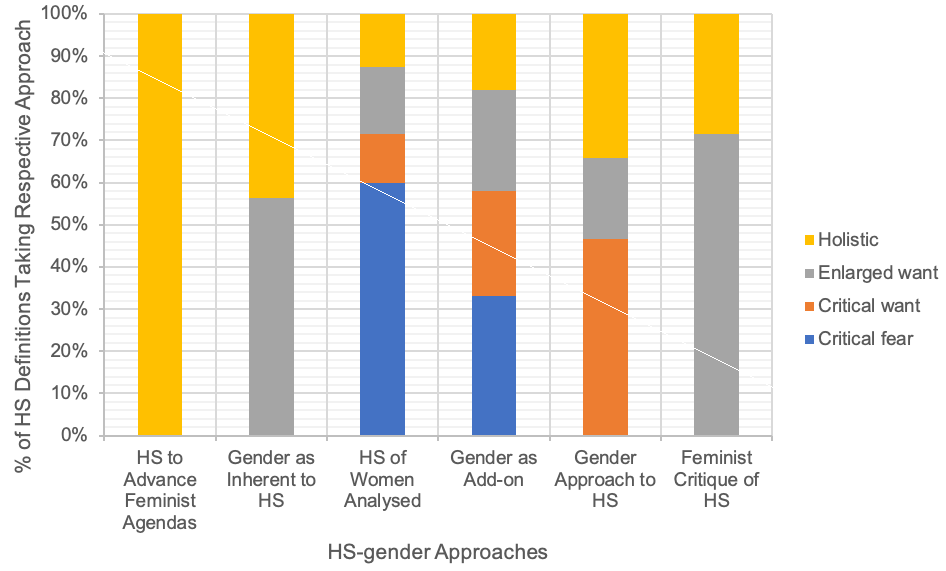
\includegraphics[width=1\textwidth]{Fig3.png}}
\captionof{figure}{Percentage of HS Definitions Taking Particular Gendered HS approach.} 
\label{Fig3}
\end{minipage}
\vspace{\baselineskip}

\begin{multicols}{2}

\subsection{Approaches' Definitions of Gender and Gender Research}

\noindent The predominant understanding of ``gender'' by any given feminist studies subcategory indicates their predominantly favored approach to HS and gender. For example, feminist study subcategories that focus on ``both'' genders all tend to favor a \textit{Gender Approach to HS}, This corresponds to  \textit{Postmodern}, \textit{Poststructural}, and \textit{Critical Feminism} in particular. 

On the other hand, feminist studies subcategories focusing on ``women'' are more scattered in their predominantly chosen approach although they favor approaches that seek \textit{Gender as an Add-on} and a \textit{HS Analysis of Women}. Studies categorized as either \textit{Mainstream}, \textit{Mainstream FSS} tend to favor both approaches equally. Only a minority of studies categorized as \textit{Critical Feminism} followed either approach which is in line with the recognition of power imbalances affecting the realization of human security, which would not be addressed by solely looking at women or adding the insecurities of women as an add-on to Human Security.

Though only three studies place themselves in the field of \textit{Ecofeminism}, the approach taken to both their conceptualization of gender as well their approaches show a much more diverse picture. Due to the limited sample size, we can therefore not assign any interpretation to this.

We therefore argue that the understanding of ``gender'' is essential to the studies' chosen gendered HS approach. Those feminist subcategories that focus on both genders in order to ask ``what does gender do?'' are largely interested in \textit{Gender Approach to HS} and thus, take a more radical rethinking of HS. Whereas those feminist subcategories that use ``gender'' to focus on women to promote the inclusion of women in their respective fields do so in order to investigate the \textit{HS of Women} or to promote \textit{Gender as an Add-on to HS}. This understanding is critical to be able to position oneself in the field of gender and human security.

\section{Conclusion}

\noindent In conclusion, four overarching HS definitions were prominent within the literature: freedom from \textit{critical fear}, freedom of \textit{critical want}, freedom to \textit{enlarged want} and a \textit{holistic} definition that calls for freedom to live life in dignity. Over the years, there has been a clear trend to increasingly move towards more holistic understandings of HS. However, when looking at their stances to Human Security in more detail, we established that most studies call for necessary additions to HS, such as power, empowerment, women, gender dimensions, the role of the state, and a more detailed discussion of the researcher's positionality. Thus, highlighting the need for a more critical look towards how gender is incorporated when studying Human Security.

\textls[-5]{When investigating the studies' used feminist studies subcategories, we identified two overarching feminist studies camps, namely, the more critical feminist approaches (i.e., \textit{Critical Feminism, Postcolonial Feminism, Postmodern Feminism}, and to a lesser extent \textit{Poststructural Feminism} and \textit{Third World Feminism}), the mainstream feminist approaches (i.e., \textit{Mainstream Feminism drawing on FSS}, and \textit{Mainstream Feminism}) and an outlier (i.e., \textit{Ecofeminism}). When assessing these feminist studies subcategories over the years, three trends emerged: (a) \textit{Critical Feminism} and \textit{Mainstream Feminism drawing on FSS} studies have steadily increased over the years, (b) \textit{Mainstream Feminist} studies have slightly decreased, and (c) studies from all other branches have remained static and minimal over the years.}

\textls[20]{When investigating studies' definitions of gender, the majority of studies used gender to refer to and focus solely on women, although a great number used gender to refer to both women and men. Only two out of ninety-five reviewed articles focused solely on men. The focus on women has increased over the years, whereas a focus on both genders decreased slightly. When relating the feminist studies subcategories back to their definition, we established that the more a study relied on critical feminist approaches, the more its usage of ``gender'' moves from ``women'' to ``both genders.''}

Out of the six different gendered HS approaches identified, the majority of studies call for a gendering of the HS paradigm by providing a \textit{Gender Approach to HS}, followed by \textit{Gender as an Add-on to HS} analyses, \textit{HS of Women}, and \textit{Gender as inherent to HS} respectively. Only a minor part of the examined literature employs a \textit{Feminist Critique of HS}, or regards \textit{HS as a tool to advance feminist agendas}.

All HS stances largely favored more gender-aware approaches, while broader HS definitions were more prevalent across more gender-aware gendered HS approaches. Those feminist studies subcategories that focus on both genders in order to ask ``what does gender do?'' were largely interested in a \textit{Gender Approach to HS} and thus a more radical rethinking of HS. Those feminist subcategories that used ``gender'' to focus on women to promote the inclusion of women in their respective fields did so in order to investigate the \textit{HS of Women} or to promote \textit{Gender as an Add-on to HS}. Thus, the findings indicate that the appropriation of ``gender'' by a study is thus heavily entangled with its chosen gendered HS approach.

This study is therefore indicative of the relevance of a critical feminist approach to address the underlying causes of human insecurity. Thus, a gendered HS approach can only challenge global (gendered) inequalities and insecurities if it fully incorporates feminist values, as proposed by critical feminist and intersectional scholars.

To further develop a critical understanding of how a gendered HS approach can enable the fulfillment of human security, we recommend a further analysis of how human security can be realized incorporating a gendered HS approach. Future research should also examine how the usage of certain sources (e.g., policy reports, studies) shapes a study's analytical focus and how this results in a consequent framing of gender and HS. Ideally, future study would relate this back to ongoing political and policy developments to understand how these may or may not affect the thinking in the field. Further, as our study identifies changing trends in the field of gender and HS, we suggest to periodically undertake a systematic review of this research field's development to ensure a representative portrayal.

\section*{Acknowledgements}
The authors would like to thank the reviewers for their valuable comments, and the participants at the Human Development and Capabilities Association at the London Conference and at WO=MEN, Dutch Gender Platform where parts of this work were presented, for their thoughtful input and discussion. 

\end{multicols}

%\vspace{\baselineskip}
\vspace*{10mm}
\begin{multicols}{2}
\renewcommand*{\refname}{\normalsize{References and Notes}}

\begin{footnotesize}
\bibliographystyle{vancouver_Librello}
\bibliography{Biblio-537}


\end{footnotesize}
\end{multicols}
\clearpage

\section{Appendix} 
\subsection{Appendix A} \label{Appendix A}

\beginsupplement

\vspace{\baselineskip}
\noindent \begin{minipage}{\columnwidth}
\centering
\resizebox{1.2\columnwidth}{!}
%\resizebox{\columnwidth}{!}
{\includegraphics[width=1\textwidth]{AFig1.jpeg}}
\captionof{figure}{Step-by-Step Flow-Diagram (Combining 2016 and 2018 Search).} 
\end{minipage}

\clearpage
\subsection{Appendix B} \label{Appendix B}

\begin{table}[H]
\centering
\begin{footnotesize}
\caption{Overview of Sample Characteristics}
\label{ATab1}
\begin{tabular}{L{5cm} L{1cm} L{1cm} L{5cm} L{1cm}}
\cline{1-2} \cline{4-5}
\cellcolor{blue!25}\textbf{Sample Characteristics} & \cellcolor{blue!25}\textbf{Count} &  & \textbf{Level of Analysis} & \\ \cline{1-2} \cline{4-5}
\textbf{Type of Study} &  &  & Community: Regional & 1 \\ \cline{1-2}
Book & 4 & & National; Regional & 1 \\
PhD Thesis & 4 &  & Regional; Global & 4 \\
Working Paper & 7 & & Community & 12 \\
Journal & 9 & & National & 13 \\
Article & 33 &  & Regional & 13 \\
Chapter & 38 &  & Global & 51 \\ \cline{1-2} \cline{4-5}
\textbf{Data Sources} &  &  & \textbf{Methodology} &  \\ \cline{1-2} \cline{4-5}
Statistical quant & 1 &  & Quantitative & 1 \\
Primary qual + descriptive quant & 2 &  & Mixed & 4 \\
Primary qual + statistical quant & 2 &  & Theory & 39 \\
Primary + secondary qual & 7 & & Qualitative & 51 \\ \cline{4-5}
Primary qual & 15 & & \textbf{Type of Analysis} & \\ \cline{4-5}
Secondary qual & 29 & & Action research & 1 \\
Theory/LR & 39 &  & Comparative analysis & 1 \\ \cline{1-2}
\textbf{Type of Data} &  &  & Descriptive statistical analysis & 1 \\ \cline{1-2}
Archival research & 1 & & Discourse analysis & 1 \\
Demographic registry & 1 & & Discourse analysis & 1 \\
Policies & 1 &  & HS analysis & 1 \\
Observations & 3 &  & Narrative analysis & 1 \\
Laws & 6 &  & Case study analysis \\
Reports & 21 &  & Statistical analysis & 2 \\
Informants & 23 &  & Discourse analysis & 4 \\
Studies/lit & 39 &  & Legal analysis & 4 \\ \cline{1-2}
\textbf{Sample Sizes} &  &  & Ethnographic analysis & 5 \\ \cline{1-2}
6-50 & 12 &  & Feminist analysis & 6 \\
229-600 & 3 &  & Policy analysis & 6 \\
1000 & 1 &  & Feminist HS analysis & 18 \\  
Not specified & 79 &  & Theoretical analysis & 41  \\ \cline{1-2} \cline{4-5}
\textbf{Geographical Focus} & & & & \\  \cline{1-2}
Western Europe & 1 & & & \\
Central Asia & 1 & & & \\
Arctic & 2 & & & \\
Eastern Europe & 3 & & & \\
Central and South America & 5 & & & \\
North America & 5 & & & \\
Middle East (incl. North Africa) & 18 & & & \\
Southeast Asia & 10 &  &  & \\
Sub-Sahara Africa & 18 &  &  & \\
N/A & 45 & & & \\ \cline{1-2}
\end{tabular}
\end{footnotesize}
\end{table}

\clearpage
\subsection{Appendix C} \label{Appendix C}

\begin{table}[H]
\centering
\begin{footnotesize}
\caption{Sample Overview of Three Articles}
\label{ATab2}
\begin{tabular}{L{3cm} L{4.2cm} L{4.2cm} L{4.2cm}}
\toprule
\textbf{Theoretical Category} & \textbf{Alexander 2010} & \textbf{Baines (2005)} & \textbf{Basch (2004)} \\ \midrule
\textbf{Gender} & \textbf{Women} & \textbf{Women} & \textbf{Women} \\ \midrule
\textit{Definition} & Uses the word gender, yet at same states that in this case it means women. Need to consider the more invisible groups, such as the women as peacemaker & ``Women's agency or relative victimization often is defined solely in relation to their gender roles and so homogenizes women's contrasting experiences of conflict where class, ethnicities, sexuality and other relations shape this experience profoundly'' (p. 8). Gender is socially constructed and subject to power dimensions. See gender equality as essential to be at peace. Her assumptions are: 1) women are more peaceful but warns that placing men solely as aggressor is not helpful, 2) women as representation of other women, 3) women both as passive victim and active subjects, 4) tends to reproduce men-women stereotypes. & Not defined clearly but focus on impact on women mainly. \\ \midrule
\textbf{Stance on Human Security} &\textbf{Ambivalent} & \textbf{Supportive but include gender} & \textbf{Critical due to its reliance on the role of the state} \\ \midrule
\textit{Assessment} & HS is a positive development although it grapples with finding solutions that are not state dependent. & It allows for a feminist approach to security but it is critical on the assumptions on gender underlying gender. While UNSCR 1325 is placed within the HS policy agenda, the article is critical on the extent it is incorporated. & It recognises the intimate connection to state security. Whose interest is really served? Who determines vital interests? \\ \midrule
\textbf{HS-gender approach} & \textbf{Gendering HS/gender approach to HS} & \textbf{Gender as add-on} & \textbf{HS of women analysed} \\ \midrule
\textit{Approach to HS and Gender} & HS ``through the intersection of militarization, gender violence and resistance in its gendered and militarized spaces'' (p. 198). To be truly successfully need to avoid conflation of gender with women as it does not allow gendered! violence to be addressed and to be truly transformative. An analysis that rejects patriarchy, racism and militarism, and allows for the transformation of `gender' is needed. It is key to accept both a range of sexualities and micro-biologies. & A feminist perspective provides new insight into the nexus between individual and structure of violence at various levels. Following Beth Woroniuk argues key issues in relation to women are missing and lack of discussion on power relations.  Some assumptions privilege gender and yet fail to address neither the larger socio-economic conditions nor the political context. More research is needed to address binary thinking, and the agenda should be situated in larger global political, economic and humanitarian regime. It needs to go beyond `add women and stir'. & Links security and empowerment in which victimisation is recognised as 2 parts of the same coin. Concern is that women are not treated as separate categories but gender issues are mainstreamed alongside all categories. \\
\bottomrule
\end{tabular}
\end{footnotesize}
\end{table}
%
%\clearpage
%
%\subsection{Appendix D} \label{Appendix D}
%
%\subsubsection{Overview of Examined Literature}
%
%\begin{itemize}
%\item Alexander, Ronni. 2010. ``Seeking Human Security in a Militarized Pacific: Struggles for Peace and Security by Pacific Island Women.'' In \textit{The Gender Imperative: Human Security vs State Security}, edited by Betty A Reardon and Asha Hans, 189–221. Routledge.
%\item Basch, Linda. 2004. ``Human Security, Globalization, and Feminist Visions.'' \textit{Peace Review} 16(1): 5–12.
%\item  Boyd, Rosalind. 2005. ``Gender and Human Security Issues: Building a Programme of Action-Research.'' \textit{Development in Practice} 15(1): 115–21. 
%\item Boyd, Rosalind. 2014. ``Locating Gender in Approaches to Human Security: an Introduction.'' In \textit{The Search for Lasting Peace: Critical Perspectives on Gender-Responsive Human Security}, edited by Rosalind Boyd, 1–17. Routledge.
%\item Bromley, Victoria. 2002. ``Human Security, Gendered Violence, and Women's Rights: Lives on the Line in the US-Mexican Borderlands.'' Carleton University.
%\item Bunch, Charlotte. 2003. ``Feminism, Peace, Human Rights and Human Security.'' \textit{Canadian Women Studies} 22(2): 6–11.
%\item Chenoy, Anuradha M. 2005. ``A Plea for Engendering Human Security.'' \textit{International Studies} 42(2): 167–79.
%\item Chenoy, Anuradha M. 2009. ``The Gender and Human Security Debate.'' \textit{IDS Bulletin} 40(2): 44–49.
%\item Chenoy, Anuradha M. 2016. ``Is Human and Gender Security Relevant for Asia?.'' In \textit{India and Emerging Asia}, edited by Sharma R, 250–67. SAGE Publications.
%\item Clough, Patricia Ticineto, and Craig Willse. 2011. ``Human Security/National Security: Gender Branding and Population Racism.'' In \textit{Beyond Biopolitics: Essays on the Governance of Life and Death}, edited by Patricia Ticineto Clough and Craig Willse, 46–64. The Duke University Press.
%\item Dankelman, Irene. 2010. ``Climate Change, Human Security and Gender.'' \textit{Gender and Climate Change an Introduction}, 12(1): 55–71.
%\item  Deiter, Connie, and Darlene Rude. 2005. ``Human Security and Aboriginal Women in Canada.'' Status of Women of Canada.
%\item Donoso, Claudia. 2016. ``Feminist Critical Human Security: Women's (in) Security and Smuggling on Ecuador's Borders.'' The University of British Columbia.
%\item Duggan, Colleen. 2014. ``Reparations for Sexual and Reproductive Violence: Gender Justice and Human Security Challenges in Guatemala and Peru.'' In \textit{The Search for Lasting Peace: Critical Perspectives on Gender-Responsive Human Security}, edited by Rosalind Boyd, 133–50. Routledge.
%\item Drysdale Walsh, Shannon. 2016. ``Advances \& Limits of Policing and Human Security for Women: Nicaragua in Comparative Perspective.'' In \textit{Gender Violence in Peace and War}, edited by Victoria Sanford, Katerina Stefatos, and Cecilia M Salvi, 133–45. Rutgers University Press.
%\item Enarson, Elaine. 2014. ``Human Security and Disasters: What a Gender Lens Offers.'' In \textit{Human Security and Natural Disasters}, edited by Christopher Hobson, Paul Bacon, and Robin Cameron, 37–56. Routledge.
%\item Erin K Baines. 2005. ``Rethinking Women, Peace and Security: a Critique of Gender in the Canadian Human Security Agenda.'' \textit{Liu Institute for Global Issues Working Paper}.
%\item Estrada-Tanck, Dorothy. 2014. ``Human Security and Women's Human Rights: Reinforcing Protection in the Context of Violence Against Women.'' 2. \textit{Rapport Centre Human Rights Working Paper Series}.
%\item Ferree, Myra Marx. 2013. ``The Discursive Politics of Gendering Human Security: Beyond the Binaries.'' In \textit{Gender, Violence, and Human Security: Critical Feminist Perspectives}, edited by Aili Mari Tripp, Myra Marx Ferree, and Christina Ewig, 285–308. New York University Press.
%\item Fox, Mary-Jane. 2004. ``Girl Soldiers: Human Security and Gendered Insecurity.'' \textit{Security Dialogue} 35(4): 465–79.
%\item Fukuda-Parr, Sakiko. 2004. ``Gender, Globalization and New Threats to Human Security.'' \textit{Peace Review} 16(1): 35–42.
%\item Gasper, Des, and Thanh-Dam Truong. 2008. ``Development Ethics Through the Lenses of Caring, Gender, and Human Security.'' 459. \textit{Institute of Social Studies Working Paper.}
%\item Gervais, Myriam. 2003. ``Human Security and Reconstruction Efforts in Rwanda.'' \textit{Development in Practice} 13(5): 542–51.
%\item Gibson, Ian R. 2004. ``Human Security Post 9-11: Gender Perspectives and Security Exclusion.'' \textit{Ritsumeikan Annual Review of International Studies} 3: 157–75.
%\item Gibson, Ian R. 2011. ``Human Security: a Framework for Peace Constructs, Gendered Perspectives and Cosmopolitan Security.'' \textit{Journal of Peace, Conflict and Development}, 17: 84–101.
%\item Gibson, Ian R, and Betty A Reardon. 2015. ``Human Security: Toward Gender Inclusion.'' In \textit{Protecting Human Security in a Post 9/11 World: Critical and Global Insights}, edited by Giorgio Shani, Makoto Sato, and Mustapha Kamal Pasha, 50–63. Palgrave Macmillan.
%\item Goldsworthy, Heather. 2010. ``Women, Global Environmental Change, and Human Security.'' In \textit{Global Environmental Change and Human Security}, edited by Richard A Matthew, Jon Barnett, Bryan McDonald, and Karen L OBrien, 215–35. Springer.
%\item Grant, J Andrew. 2014. ``Human Security and the G-8 Action Plan: What Provisions for Women and Children in Post-Conflict Communities?.'' In \textit{The Search for Lasting Peace: Critical Perspectives on Gender-Responsive Human Security}, edited by Rosalind Boyd, 151–68. Routledge.
%\item Groves, Gabrielle Eva Carol, P Resurreccion Bernadette, and Philippe Doneys. 2009. ``Keeping the Peace Is Not Enough: Human Security and Gender-Based Violence During the Transitional Period of Timor-Leste.'' \textit{Journal of Social Issues in Southeast Asia} 24(2): 186–210.
%\item Gupta, Sanju. 2012. ``Human Security, Conflict and Women: Rwanda in Retrospect.'' \textit{International Journal of Interdisciplinary Social Sciences} 6(10): 191–201.
%\item Gupta, Sonika. 2003. ``Human Security, Economic Development and Gender.'' In \textit{Human Security in South Asia: Energy, Gender, Migration, and Globalisation}, edited by P R Chari and Sonika Gupta, 52–66. Berghahn Books.
%\item Hayes, Anna M. 2007. ``Women's Vulnerability to HIV/AIDS in China:
%a Case Study for the Engendering of Human Security Discourse.'' University of Southern Queensland.
%\item Henriquez, Narda, and Christina Ewig. 2013. ``Integrating Gender Into Human Security: Peru's Truth and Reconciliation Commission.'' In \textit{Gender, Violence, and Human Security: Critical Feminist Perspectives}, edited by Aili Mari Tripp, Myra Marx Ferree, and Christina Ewig, 260–84. New York University Press.
%\item Hoogensen, Gunhild. 2005. ``Gender, Identity, and Human Security: Can We Learn Anything From the Case of Women Terrorists?.'' \textit{Canadian Foreign Policy Journal?} 12(1): 119–40.
%\item Hoogensen, Gunhild. 2009. ``Gender, Human Security and Northern Fisheries.'' In \textit{Gender, Culture and Northern Fisheries}, edited by Joanna Kafarowski, 219–34. The University of Alberta Press.
%\item Hoogensen, Gunhild, and Kirsti Stuv{\o}y. 2006. ``Gender, Resistance and Human Security.'' Security Dialogue 37(2): 207–28.
%\item Hudson, Heidi. 2005. ```Doing' Security as Though Humans Matter: a Feminist Perspective on Gender and the Politics of Human Security.'' \textit{Security Dialogue} 36(2): 155–74.
%\item  Hudson, Heidi. 2006. ``Human Security and Peacebuilding Through a Gender Lens: Challenges of Implementation in Africa.'' 37. \textit{DIIS Working Paper}.
%\item Hudson, Heidi. 2011. ``Inhabitants of Interstices? Feminist Analysis at the Intersection of Peace Studies, Critical Security Studies and Human Security.'' \textit{Strategic Review for Southern Africa} 33(2): 26–50.
%\item Hudson, Natalie F. 2009. \textit{Gender, Human Security and the United Nations: Security Language as a Political Framework for Women}. Routledge.
%\item Hudson, Natalie F. 2013. ``Evolving Threats and Faceless Enemies: Engendering Human Security in the UN.'' University of Connecticut.
%\item Irlbacher-Fox, Stephanie, Jackie Price, and Elana Wilson Rowe. 2014. ``Women's Participation in Decision Making: Human Security in the Canadian Arctic.'' In \textit{Environmental and Human Security in the Arctic}, edited by Gunhild Hoogensen, Dawn R Bazely, Marina Goloviznina, and Andrew J Tanentzap, 203–30. Routledge.
%\item Isike, Christopher, and Kwame Owusu-Ampomah. 2017. ``A Human Security Analysis of the Situation of Girls and Young Women in Kwazu-Natal, South Africa.'' \textit{African Population Studies} 31(1): 3179–93.
%\item Jamal, Manal A. 2014. ``The Palestinian Women's Sector and the Promotion of Human Security.'' In \textit{The Search for Lasting Peace: Critical Perspectives on Gender-Responsive Human Security}, edited by Rosalind Boyd, 89–102. Routledge.
%\item Jayaweera, Hiranthi. 2017. ``Access to Healthcare for Vulnerable Migrant Women in England: a Human Security Approach.'' \textit{Current Sociology}, 66: 273–85.
%\item Khattak, Saba Gul, Kiran Habib, and Foqia Sadiq Khan. 2008. ``Women and Human Security in South Asia: the Cases of Bangladesh and Pakistan.'' \textit{SDPI Working Paper}.
%\item Kinney, Edith. 2013. ``Securitizing Sex, Bodies, and Borders: the Resonance of Human Security Frames in Thailand's `War Against Human Trafficking'.'' In \textit{Gender, Violence, and Human Security: Critical Feminist Perspectives}, edited by Aili Mari Tripp, Myra Marx Ferree, and Christina Ewig, 79–108. New York University Press.
%\item Lammers, Ellen. 1999. \textit{Refugees, Gender and Human Security: a Theoretical Introduction and Annotated Bibliography}. International Books.
%\item Lewis, Desiree. 2006. ``Rethinking Human Security: the Implications of Gender Mainstreaming.'' In \textit{From State Security to Human Security in Southern Africa: Policy Research and Capacity Building Challenges}, edited by Cheryl Hendricks, 9–17. ISS Monograph Series.
%\item Lukunka, Barbra. 2011. ``New Big Men: Refugee Emasculation as a Human Security Issue.'' \textit{International Migration} 50(5): 130–41.
%\item Marhia, Natasha. 2013. ``Some Humans Are More Human Than Others: Troubling the `Human' in Human Security from a Critical Feminist Perspective.'' \textit{Security Dialogue} 44(1): 19–35. 
%\item McFee, Deborah. 2017. ``Women/Gender and Development in Trinidad and Tobago and Post-Genocide Rwanda: Complicating Human Security, Carving Out a National Gender Policy Response to Violence Against Women.'' \textit{Caribbean Review of Gender Studies} 11: 83-110.
%\item McKay, Susan. 2004. ``Women, Human Security, and Peacebuilding: a Feminist Analysis.'' In \textit{Conflict and Human Security a Search for New Approaches of Peacebuilding}, 152–75.
%\item Moghadam, Valentine M. 2011. ``Afghanistan: Are Human Security and Gender Justice Possible?.'' \textit{Works and Days} 29: 1–18.
%\item Moghadam, Valentine M. 2013. ``Toward Human Security and Gender Justice: Reflections on Afghanistan and Iraq.'' In \textit{Globalization, Social Movements, and Peacebuilding}, edited by Jackie Smith, 97–130. Syracuse.
%\item Moussa, Ghada. 2008. ``Gender Aspects of Human Security.'' \textit{International Social Science Journal} 59(1): 81–100.
%\item Muthien, Bernedette. 2000. ``Human Security Paradigms Through a Gendered Lens.'' \textit{Agenda: Empowering Women for Gender Equity}, 43: 46–56.
%\item Muthien, Bernedette. 2010. ``Human Security and Intersectional Oppressions: Women in South Africa.'' In \textit{The Gender Imperative: Human Security vs State Security}, edited by Betty A Reardon and Asha Hans, 59–82. Routledge.
%\item Nuruzzaman, Mohammed. 2006. ``Paradigms in Conflict: the Contested Claims of Human Security, Critical Theory and Feminism.'' \textit{Cooperation and Conflict} 41(3): 285–303. 
%\item O'Manique, Colleen, and Sandra J MacLean. 2011. ``Pathways Among Human Security, Gender, and HIV/AIDS in Sub-Saharan Africa.'' \textit{Canadian Journal of African Studies/Revue Canadienne Des Études Africaines} 44(3) : 457–78.
%\item Okotie, Henry V. 2007. ``Gender, Conflict and Human Security in Nigeria: Challenges and Prospects.'' \textit{Gender and Behaviour} 5(2): 1421–33.
%\item Oswald Spring, Ursula. 2018. ``Human, Gender and Environmental Security at Risk from Climate Change.'' In \textit{Preventing Health and Environmental Risks in Latin America}, edited by M L Marvan and E Lopez-Vazquez, 23:167–92. Springer.
%\item Ozolina, Zaneta, ed. 2015. \textit{Gender and Human Security: A View From the Baltic Sea Region}. Zinatne Publishers.
%\item Panda, Snehalata. 2015. ``Disempowerment of Tribal Women: A Human Security Perspective.'' \textit{Local Government Quaterly} 85(1): 27–39.
%\item Parmar, Parveen Kaur, Pooja Agrawal, Ravi Goyal, Jennifer Scott, and P Gregg Greenough. 2014. ``Need for a Gender-Sensitive Human Security Framework: Results of a Quantitative Study of Human Security and Sexual Violence in Djohong District, Cameroon.'' \textit{Conflict and Health} 8(6): 1–12.
%\item Pividori, Claudia, and Paola Degani. 2018. ``Reflecting on Criminalizing Male Violence Against Women Under Human Rights and Human Security Discourses: A Feminist Legal and Policy Analysis.'' Global Jurist 19(1): 1–12. 
%\item Radu, Mihaela. 2015. ``Gender Equality: A Condition for Achieving Human Security.'' \textit{Strategic Impact}, 2: 104–11.
%\item Randriamaro, Zo. 2012. ``Whose Human Security? Gender, Neoliberalism and the Informal Economy of Sub-Saharan African.'' In \textit{Gendered Insecurities, Health and Development in Africa}, 72–97. Routledge.
%\item Reardon, Betty A. 2010. ``Women and Human Security: A Feminist Framework and Critique of the Prevailing Patriarchal Security System.'' In \textit{The Gender Imperative: Human Security vs State Security}, edited by Betty A Reardon and Asha Hans, 7–36. Routledge.
%\item Reardon, Betty A, and Asha Hans. 2010. ``Conclusion: Framing a Gender and Human Security Discourse: Initiating the Inquiry.'' In \textit{The Gender Imperative: Human Security vs State Security}, 410–26. Routledge.
%\item Reardon, Betty A, and Dale T Snauwaert. 2015. ``Women and Human Security: A Feminist Framework and Critique of the Prevailing Patriarchal Security System.'' In \textit{Betty a. Reardon Key Texts in Gender and Peace}, 109–28. Springer.
%\item Robinson, Fiona. 2011. \textit{The Ethics of Care: A Feminist Approach to Human Security}. Philadelphia: Temple University Press.
%\item Rosenow-Williams, Kerstin, and Katharina Behmer. 2015. ``A Gendered Human Security Perspective on Humanitarian Action in IDP and Refugee Protection.'' \textit{Refugee Survey Quarterly} 34(3): 1–23.
%\item Rubio-Marin, Ruth, and Dorothy Estrada-Tanck. 2013. ``Violence Against Women, Human Security, and Human Rights of Women and Girls: Reinforced Obligations in the Context of Structural Vulnerability.'' In \textit{Gender, Violence, and Human Security: Critical Feminist Perspectives}, edited by Aili Mari Tripp, Myra Marx Ferree, and Christina Ewig, 238–59New York University Press.
%\item Sasaki, Shinobu, Kyoko Kusakabe, and Philippe Doneys. 2015. ``Exploring Human (in-)Security from a Gender Perspective: a Case Study of Subcontracted Workers in Thailand.'' \textit{International Journal of Sociology and Social Policy} 36(5/6): 304–18.
%\item Songsore, Jacob. 2012. ``Gender, Environment and Human Security in the Greater Accra Metropolitan Area (GAMA), Ghana.'' In \textit{Gendered Insecurities, Health and Development in Africa}, edited by Howard Stein and Amal Hassan Fadlalla, 131–53. Routledge.
%\item Spring, Ursula Oswald. 2008. ``Gender and Disasters: Human, Gender and Environmental Security---a HUGE Challenge.'' \textit{Source} 8. UNU-EHS.
%\item Spring, Ursula Oswald. 2009. ``A HUGE Gender Security Approach: Towards Human, Gender, and Environmental Security.'' In Facing Global Environmental Change: Environmental, Human, Energy, Food, Health and Water Security Concepts, edited by Hans Günter Brauch, Ursula Oswald Spring, John Grin, Czeslaw Mesjasz, Patricia Kameri-Mbote, Navnita Chadha Behera, Bechir Chourou, and Heinz Krummenacher, 1157–81. Heidelberg.
%\item Stuv{\o}y, Kirsti. 2010. ``Human Security Research Practices: Conceptualizing Security for Women's Crisis Centres in Russia.'' \textit{Security Dialogue} 41(3): 279–99.
%\item Stuv{\o}y, Kirsti. 2014. ``Human Security and Women's Security Reality in Northwest Russia.'' In \textit{Environmental and Human Security in the Arctic}, edited by Gunhild Hoogensen, Dawn R Bazely, Marina Goloviznina, and Andrew J Tanentzap, 231–49. Routledge.
%\item Summerfield, Gale. 2015. ``Gender, Global Crises, and Human Security.'' In \textit{Human Security, Changing States and Global Responses: Institutions and Practices}, edited by Sangmin Bae and Makoto Maruyama, 88–102. Routledge.
%\item Svensson, Katja. 2010. ``Human Security as Inclusive Security---Gender, Epistemology and Equality.'' \textit{African Security Review} 16(2): 1–13.
%\item Sweet, Victoria. 2014. ``Extracting More Than Resources: Human Security and Arctic Indigenous Women.'' \textit{Seattle University Law Review} 37: 1221–43.
%\item Taylor, Viviene. 2004. ``From State Security to Human Security and Gender Justice.'' \textit{Agenda: Empowering Women for Gender Equity}, 65–70.
%\item Thomas, Lahoma, and Rebecca Tiessen. 2011. ``Human Security, Gender-Based Violence and the Spread of HIV/AIDS in Africa: a Feminist Analysis.'' \textit{Canadian Journal of African Studies / Revue Canadienne Des Études Africaines} 44(3): 479–502.
%\item Tiessen, Rebecca, Jane Parpart, and Miriam Grant. 2010. ``Gender, HIV/AIDS, and Human Security in Africa.'' \textit{Canadian Journal of African Studies/Revue Canadienne Des Études Africaines} 44(3): 449–56. 
%\item Timothy, Kristen. 2007. ``Engendering Human Security: Intersections of Security, Globalization and Gender.'' In \textit{Unpacking Globalisation Markets, Gender, and Work}, edited by Linda E. Lucas, 47–57. Lexington Books.
%\item Tripp, Aili Mari. 2013. ``Toward a Gender Perspective on Human Security.'' In \textit{Gender, Violence, and Human Security: Critical Feminist Perspectives}, edited by Aili Mari Tripp, Myra Marx Ferree, and Christina Ewig, 3-32. New York University Press.
%\item Truong, Thanh-Dam. 2009a. ``Feminist Knowledge and Human Security: Bridging Rifts Through the Epistemology of Care.'' \textit{ISS Working Paper} 481.
%\item Truong, Thanh-Dam. 2009b. ``Human Security and the Governmentality of Neo-Liberal Mobility: a Feminist Perspective.'' In \textit{Facing Global Environmental Change: Environmental, Human, Energy, Food, Health and Water Security Concepts}, edited by Hans Günter Brauch, Ursula Oswald Spring, John Grin, Czeslaw Mesjasz, Patricia Kameri-Mbote, Navnita Chadha Behera, and Heinz Krummenacher, 1183–89. Springer.
%\item Truong, Thanh-Dam, Saskia Wieringa, and Amrita Chhachhi. 2007. ``Introduction: Gender Questions in the Human Security Framework.'' In \textit{Engendering Human Security Feminist Perspectives}, edited by Thanh-Dam Truong, Saskia Wieringa, and Amrita Chhachhi, ix–xxx. Zed Books.
%\item Uddin, M Bashir. 2014. ``Human Trafficking in South Asia: Issues of Corruption and Human Security.'' \textit{International Journal of Social Work and Human Services Practice} 2(1): 18–27.
%\item Uddin, M Bashir. 2017. ``Revisiting Gender-Sensitive Human Security Issues and Human Trafficking in South Asia: The Cases of India and Bangladesh.'' In \textit{Crime, Criminal Justice, and the Evolving Science of Criminology in South Asia}, edited by Shahid M Shahidullah, 219–245. Palgrave McMillan.
%\item Valasek, Kristin. 2014. ``Please Leave Your Weapons at the Door: Re-Gendering Human Security From Human Security Now To Disarmament.'' In \textit{The Search for Lasting Peace: Critical Perspectives on Gender-Responsive Human Security}, edited by Rosalind Boyd, 21–28. Routledge.
%\item Youssef, Maisaa. 2008. ``Suffering Men of Empire: Human Security and the War on Iraq.'' \textit{Cultural Dynamics} 20(2): 149–66. 
%\end{itemize}

\end{document}